\subsection{Structured-Control-Flow Construct}
\label{section:mir-translation-cfg-construct}

Translating from stack-based IR to register-based IR is not trivial, especially
when non-linear control flow structures appeared. This problem appeared in many
runtime system implementations, such as Numba \cite{numba}, a just-in-time (JIT)
compiler for Python. Usually, one needs some algorithm to recover the control
flow structure from annoying jump instructions. Luckily, in WebAssembly, we can
translate the stack-based bytecode into register-based basic blocks in linear
time, thanks to the structured control flow constructs and their validation
rules defined in WebAssembly. In this section, we will cover the translation
patterns used for WebAssembly's structured-control-flow constructs, namely
\texttt{block}, \texttt{if} and \texttt{loop}.

\begin{figure}
  \centering
  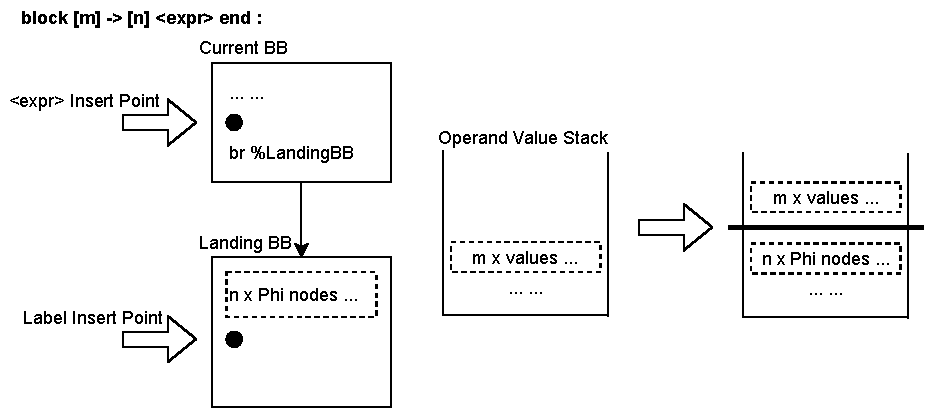
\includegraphics[width=\textwidth]{Images/4.MIR/translate-block.pdf}
  \caption{WebAssembly \texttt{block} translation pattern}
  \label{fig:translate-block}
\end{figure}

\paragraph{Block}
In the background chapter, we provide a general illustration of the three
structured control flow constructs. As a quick recap, \texttt{block} is the
simplest form of a structured control flow construct. It implicitly introduces
a label at the end of its enclosing instructions. A branch instruction
referring to this label will redirect the control flow to the end of the block.
Figure~\ref{fig:translate-block} illustrates the translation pattern for
WebAssembly \texttt{block} in SableWasm MIR. We will first clarify some of the
terminologies we used in the figure, and we will use the same terms later in
the \texttt{loop} and \texttt{if} pattern discussion for consistency.
\emph{Expr Insert Point} refer to the starting position for the generated
instructions when we recursively translate the instructions within the enclosing
expression of the \texttt{block} instruction. Furthermore,
\emph{Label Insert Point} refer to the position for generated instructions when
we finish the recursive translation and resume to the parent expression of the
\texttt{block} instruction. A \emph{label stack entry} is a tuple consisting of
a pointer to the landing basic block, a list of $\phi$ nodes expecting merge
values, and a pointer to the \emph{label insert point}. The translation pattern
for \texttt{block} is pretty simple; we continue on the current basic block and
prepare the landing basic block for the block instruction as a branch
instruction within the expression may refer to the label. Additionally, to fully
support multi-value extension in WebAssembly, we also need to prepare the $\phi$
nodes in the landing basic block. SableWasm generates the $\phi$ nodes based on
the type of the \texttt{block} instruction. WebAssembly validation rules ensure
that the expression within the \texttt{block} can access exactly $m$ values from
the stack and put $n$ values onto the stack. Finally, we will append an
unconditional branch to the landing basic block because in WebAssembly,
if the control flow reaches the bottom of the \texttt{block} expressions, it
will implicitly fall through. For the operand stack, we will first pop $m$
values from the stack as \texttt{block} instruction's type suggests and push the
$\phi$ nodes as the result values. Then, we need to set up the boundary between
the operand stack for the expression contained within the \texttt{block}.
Figure~\ref{fig:translate-block} represents this with the bold line in the
result operand value stack. The last step is to push the $m$ values back to the
stack, as they are passed to the expression within the \texttt{block}.

\begin{figure}
  \centering
  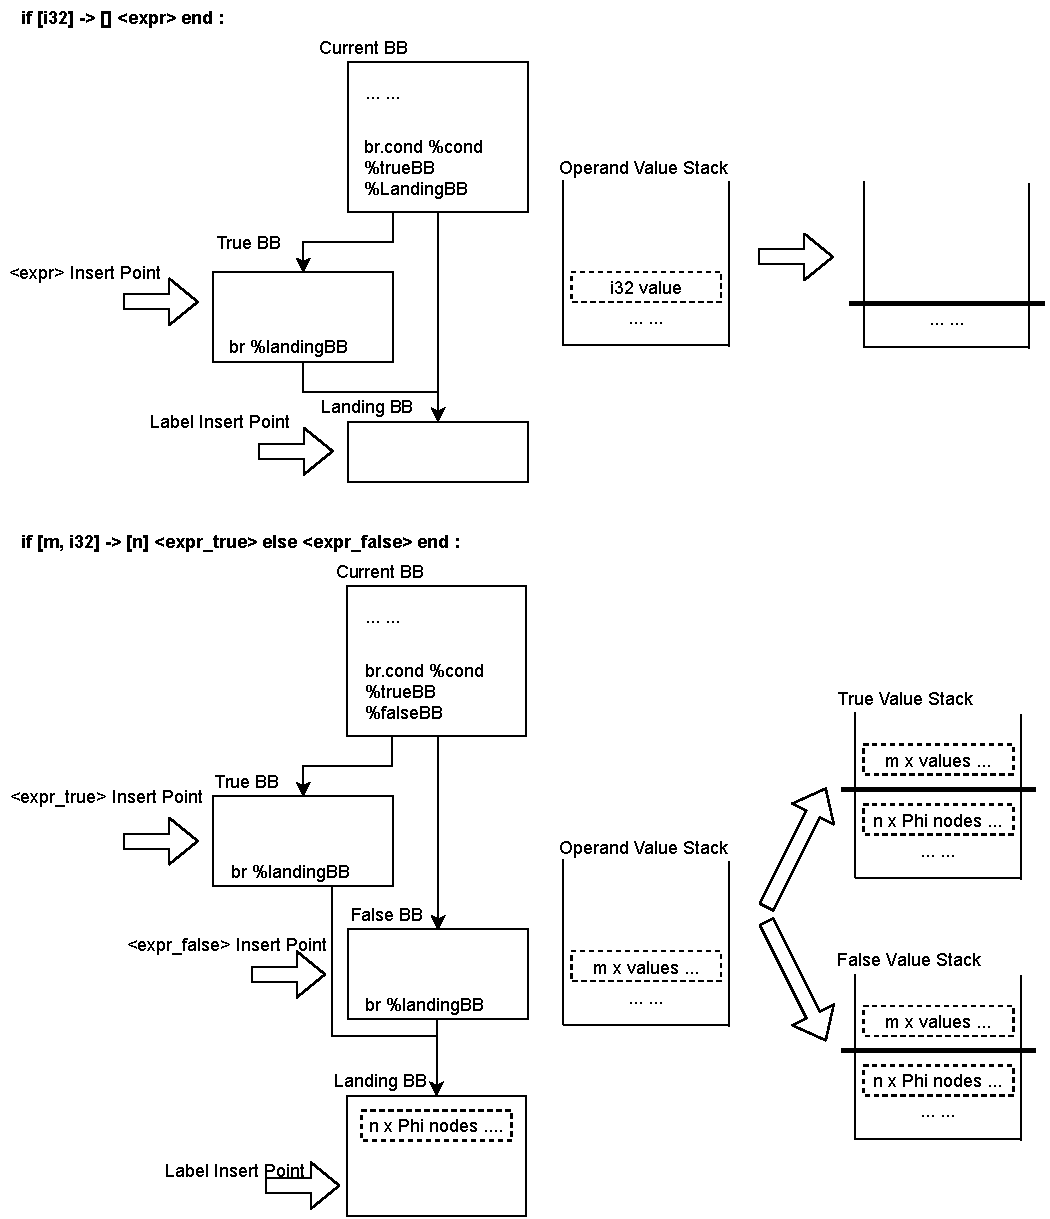
\includegraphics[width=\textwidth]{Images/4.MIR/translate-if.pdf}
  \caption{WebAssembly \texttt{if} translation pattern}
  \label{fig:translate-if}
\end{figure}

\paragraph{If}
The next control-flow structure defined WebAssembly is \texttt{if}.
WebAssembly's \texttt{if} is an expression instead of a statement that appears
in many other languages such as C. The \texttt{if} expression can yield some
values indicated by its type. Figure~\ref{fig:translate-if} illustrates the
translation patterns in SableWasm. There are two types of \texttt{if}
instruction defined in WebAssembly specification. The first case is a `partial'
\texttt{if} instruction, where it only contains the `true' branch. From
WebAssembly validation rules, it's easy to show that the only possible type is
\texttt{[i32]->[]}, even with the multi-value extension proposal. This implies
that the expression within the \texttt{if} instruction must start with an empty
operand stack. Hence, the translation pattern for the partial \texttt{if} is
quite straightforward: we only need to pop the condition value from the operand
stack and construct a conditional branch based on this value in the current
basic block. On the other hand, we also have `full' \texttt{if} instructions
with both `true' and `false' expressions. The validation rules ensure that both
expressions must have the same type. The translation pattern is more complex
compare to that of a `partial' \texttt{if}. In this case, we have to prepare the
landing basic block similar to what we did for the \texttt{block} construct.
We need to generate $n$ $\phi$ nodes for data-flow mergers from the `true'
branch, the `false' branch, and any possible branch instruction within both
nested expressions. Similarly, we need to pop $m$ values from the stack for
operand values stack and then push $n$ $\phi$ nodes. And, within both nested
expressions, push $m$ values back to the stack.

\begin{figure}
  \centering
  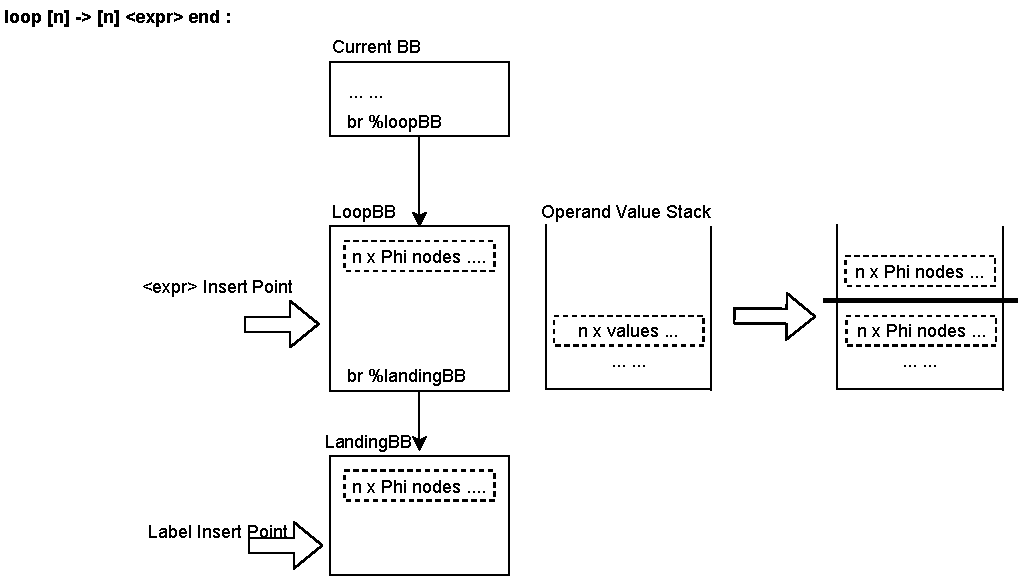
\includegraphics[width=\textwidth]{Images/4.MIR/translate-loop.pdf}
  \caption{WebAssembly \texttt{loop} translation pattern}
  \label{fig:translate-loop}
\end{figure}

\paragraph{Loop}
The last control-flow structure defined in WebAssembly is \texttt{loop}.
Figure~\ref{fig:translate-loop} gives a general illustration of SableWasm's
translation pattern for \texttt{loop} instructions. Similar to the `partial'
\texttt{if} we discussed in the previous paragraph, one can show that, under
WebAssembly's validation rules, the parameter types for the \texttt{loop}
instruction must equal to the result types. The \texttt{loop} instruction is
similar to the \texttt{block} instruction, except that if any branch
instruction refers to it, the branch instruction should transfer the control
flow to the start of the expression within the instruction instead of the end.
Thus, we need to prepare a standalone basic block for the nested expression in
\texttt{loop}, along with the $\phi$ nodes to merge value on each loop
iteration. Note that we also introduce $\phi$ nodes in the landing basic block.
One may argue that there is no need for these $\phi$ nodes, as only one block
can reach the loop exit, and no value merging will occur. Indeed, these
$\phi$ nodes will always be trivial $\phi$ nodes, which have only one
possible value inflow. However, this is due to the limitation of our translation
framework.

In this section, we discussed the translation patterns for WebAssembly
structured control flow constructs. Thanks to WebAssembly validation rules, the
types for these structured control flow instructions explicitly mark value
merging and imply possible $\phi$ nodes. Furthermore, one can show that the
control graph generated above is indeed in SSA form. However, the directly
generated control flow graph is not easily understandable by users. This mainly
comes from two facts. First, the WebAssembly-targeting compiler may generate
awkward patterns to fit in the structured control-flow constructs. Second,
SableWasm translation patterns for structured-control flow constructs are not
optimal.